\documentclass[tikz, border=20pt]{standalone}
\usepackage{helvet}
\renewcommand{\familydefault}{\sfdefault}
\usetikzlibrary{shapes.geometric, arrows.meta, positioning, fit, calc, backgrounds}

\begin{document}
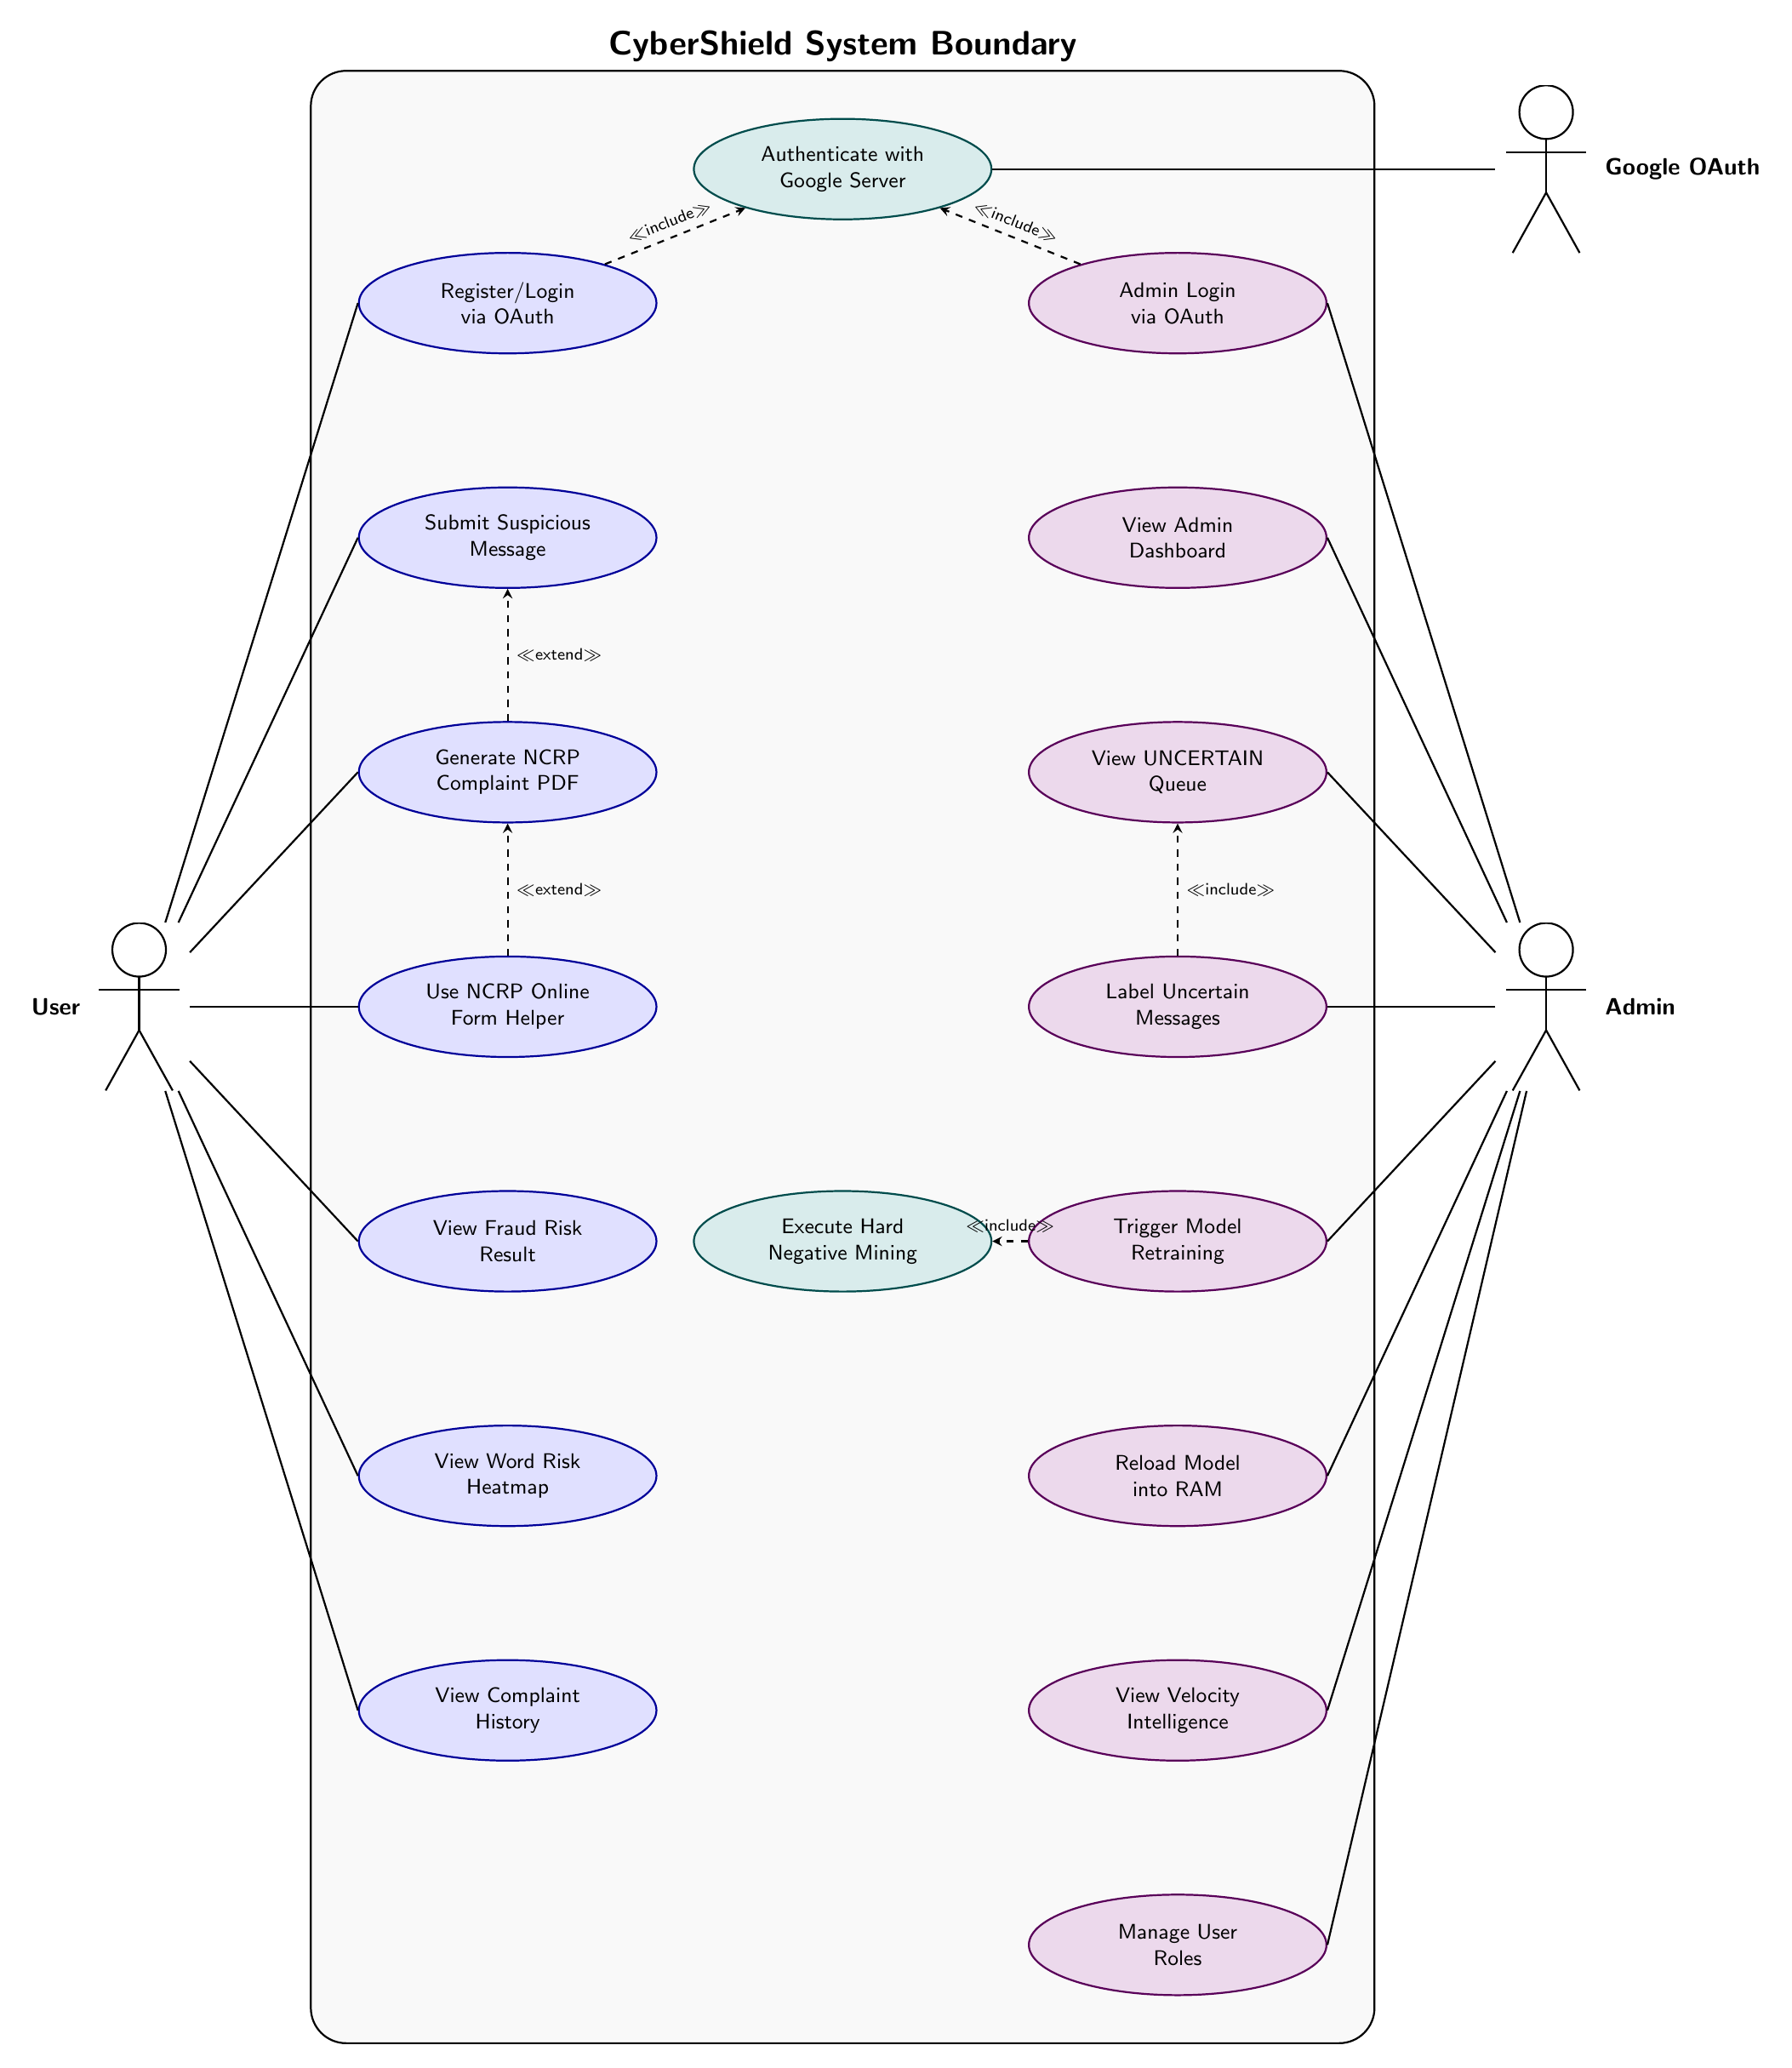
\begin{tikzpicture}[
  actor/.style={
    inner sep=0pt,
    minimum width=1.5cm,
    minimum height=2.5cm,
    path picture={
      \draw[thick] (path picture bounding box.north) ++(0,-0.4) circle (0.4); % Head
      \draw[thick] (path picture bounding box.north) ++(0,-0.8) -- ++(0,-0.8); % Body
      \draw[thick] (path picture bounding box.north) ++(-0.6,-1.0) -- ++(1.2,0); % Arms
      \draw[thick] (path picture bounding box.north) ++(0,-1.6) -- ++(-0.5,-0.9); % Left Leg
      \draw[thick] (path picture bounding box.north) ++(0,-1.6) -- ++(0.5,-0.9); % Right Leg
    }
  },
  usecase/.style={
    ellipse, draw=black, thick, align=center,
    text width=3.0cm, minimum height=1.5cm, inner sep=2pt, font=\small, fill=white
  },
  citizencase/.style={
    ellipse, draw=blue!60!black, thick, align=center,
    text width=3.0cm, minimum height=1.5cm, inner sep=2pt, font=\small, fill=blue!12
  },
  admincase/.style={
    ellipse, draw=violet!70!black, thick, align=center,
    text width=3.0cm, minimum height=1.5cm, inner sep=2pt, font=\small, fill=violet!15
  },
  sharedcase/.style={
    ellipse, draw=teal!60!black, thick, align=center,
    text width=3.0cm, minimum height=1.5cm, inner sep=2pt, font=\small, fill=teal!15
  },
  extend/.style={->, dashed, thick, >=stealth},
  include/.style={->, dashed, thick, >=stealth},
  communicate/.style={-, thick, draw=black}
]

% ----------------- ACTORS -----------------
\node[actor, label={[font=\bfseries]left:User}] (user) at (-5.5, -10.5) {};
\node[actor, label={[font=\bfseries]right:Admin}] (admin) at (15.5, -10.5) {};
\node[actor, label={[font=\bfseries]right:Google OAuth}] (google) at (15.5, 2) {};

% ----------------- CITIZEN USE CASES -----------------
\node[citizencase] (uc_reg) at (0, 0) {Register/Login\\via OAuth};
\node[citizencase] (uc_sub) at (0, -3.5) {Submit Suspicious\\Message};
\node[citizencase] (uc_pdf) at (0, -7) {Generate NCRP\\Complaint PDF};
\node[citizencase] (uc_hlp) at (0, -10.5) {Use NCRP Online\\Form Helper};
\node[citizencase] (uc_res) at (0, -14) {View Fraud Risk\\Result};
\node[citizencase] (uc_map) at (0, -17.5) {View Word Risk\\Heatmap};
\node[citizencase] (uc_his) at (0, -21) {View Complaint\\History};

% ----------------- ADMIN USE CASES -----------------
\node[admincase] (uc_alog) at (10, 0) {Admin Login\\via OAuth};
\node[admincase] (uc_dash) at (10, -3.5) {View Admin\\Dashboard};
\node[admincase] (uc_que) at (10, -7) {View UNCERTAIN\\Queue};
\node[admincase] (uc_lab) at (10, -10.5) {Label Uncertain\\Messages};
\node[admincase] (uc_ret) at (10, -14) {Trigger Model\\Retraining};
\node[admincase] (uc_rel) at (10, -17.5) {Reload Model\\into RAM};
\node[admincase] (uc_vel) at (10, -21) {View Velocity\\Intelligence};
\node[admincase] (uc_rol) at (10, -24.5) {Manage User\\Roles};

% ----------------- SHARED / INCLUDED USE CASES -----------------
\node[sharedcase] (uc_auth) at (5, 2) {Authenticate with\\Google Server};
\node[sharedcase] (uc_hnm)  at (5, -14) {Execute Hard\\Negative Mining};

% ----------------- SYSTEM BOUNDARY -----------------
\begin{scope}[on background layer]
    \node[draw=black, thick, rounded corners=15pt, fill=gray!5, inner sep=20pt,
          fit=(uc_reg) (uc_sub) (uc_pdf) (uc_hlp) (uc_res) (uc_map) (uc_his)
              (uc_alog) (uc_dash) (uc_que) (uc_lab) (uc_ret) (uc_rel) (uc_vel) (uc_rol)
              (uc_auth) (uc_hnm)] (system) {};
    \node[anchor=south, font=\bfseries\Large, text=black] at (system.north) {CyberShield System Boundary};
\end{scope}

% ----------------- ACTOR TO USE CASE CONNECTIONS -----------------
\draw[communicate] (user) -- (uc_reg.west);
\draw[communicate] (user) -- (uc_sub.west);
\draw[communicate] (user) -- (uc_res.west);
\draw[communicate] (user) -- (uc_map.west);
\draw[communicate] (user) -- (uc_pdf.west);
\draw[communicate] (user) -- (uc_hlp.west);
\draw[communicate] (user) -- (uc_his.west);

\draw[communicate] (admin) -- (uc_alog.east);
\draw[communicate] (admin) -- (uc_dash.east);
\draw[communicate] (admin) -- (uc_que.east);
\draw[communicate] (admin) -- (uc_lab.east);
\draw[communicate] (admin) -- (uc_ret.east);
\draw[communicate] (admin) -- (uc_rel.east);
\draw[communicate] (admin) -- (uc_vel.east);
\draw[communicate] (admin) -- (uc_rol.east);

% Secondary Actor Connection
\draw[communicate] (uc_auth.east) -- (google.west);

% ----------------- INCLUDE / EXTEND RELATIONSHIPS -----------------
\draw[include] (uc_reg) -- node[above, sloped, font=\scriptsize] {$\ll$include$\gg$} (uc_auth);
\draw[include] (uc_alog) -- node[above, sloped, font=\scriptsize] {$\ll$include$\gg$} (uc_auth);

\draw[extend] (uc_pdf) -- node[right, font=\scriptsize] {$\ll$extend$\gg$} (uc_sub);
\draw[extend] (uc_hlp) -- node[right, font=\scriptsize] {$\ll$extend$\gg$} (uc_pdf);

\draw[include] (uc_lab) -- node[right, font=\scriptsize] {$\ll$include$\gg$} (uc_que);
\draw[include] (uc_ret) -- node[above, font=\scriptsize] {$\ll$include$\gg$} (uc_hnm);

\end{tikzpicture}
\end{document}
